\documentclass[tikz,border=1cm]{standalone}

\usepackage{tikz,pgfplots}

\usetikzlibrary{decorations.shapes}
\usetikzlibrary{arrows.meta,calc,decorations.markings,math,arrows.meta}
\usetikzlibrary{%
    decorations.pathreplacing,%
    decorations.pathmorphing%
}


%------------   Todo está en 2D porque no entiendo 3D   :c    ------------%


\begin{document}
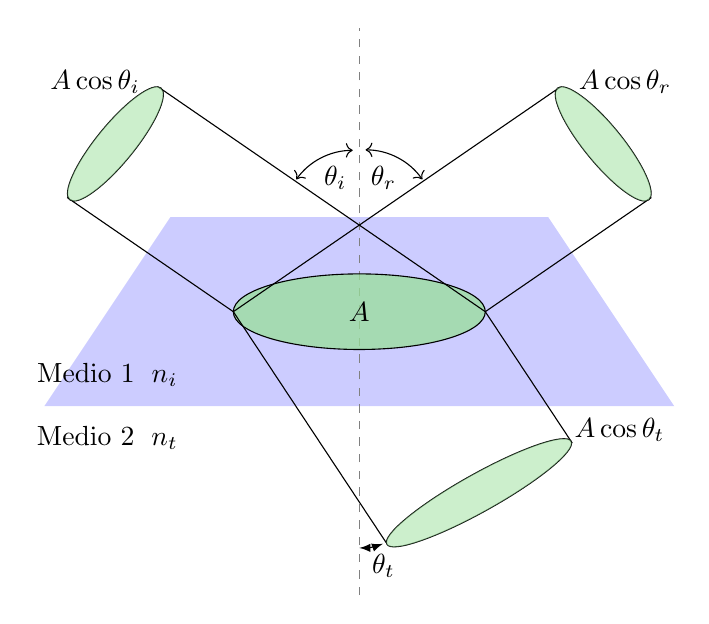
\begin{tikzpicture}[scale=.8]
%\draw (3.46,1.9) circle(2pt);ESTA ES LAREFERENCIA PARA ANTES DE MOVER LAS COSAS

%---------------------------------------------------------------------------------------- SUPERFICIE
\fill[blue!20]			
(-5,-1) -- (-3,2) 
-- (3,2) -- (5,-1)
--(-5,-1);						

\draw[dashed,gray](0,-4)--(0,5);  %---------------------------------------------------- Vertical dashed line

\node at (-4,-.5) {Medio 1 $\; n_i$}; %-------------------------------------------------- media names
\node at (-4,-1.5) {Medio 2 $\; n_t$};

%---------------------------------------------------------------------------------------- SPOT INTERFAZ
\fill[green!70!black!40, opacity= .75] (0,.5) circle (2 and .6); 
\draw[black](0,.5) circle (2 and .6)		% -------------------------------------------  Etiqueta área
			(0,.5)node[]{$A$};	
%---------------------------------------------------------------------------------------- INCIDENTE
\path[shift = {(0,1.7)}] (0,0)++(112.5:1cm)node{$\theta_i$};   %------------------------- Angle
\draw[<->,shift = {(0,2.1)}](-1,.5)arc(144.5:90:1.1cm);

\draw [-,shift = {(-2,.5)}, rotate = 55.5] (0,0) -- (0,3.2);   %------------------------- Cara del cilindro(Rota desde 90°)
\draw[-, shift = {(2,.5)},rotate = 55.5] (0,0) -- (0,6.3);

\draw[black, rotate = 50.75, shift = {(0,5)}](0,0) circle (1.145 and .3)		%-------- Tapa del cilidndro del del área
											  (1.1,.2)node[left]{ $A\cos\theta_i$};
\fill[green!70!black!40, opacity= .5, rotate = 50.75, shift = {(0,5)}](0,0) circle (1.145 and .3);

%---------------------------------------------------------------------------------------- REFLEJADO
\path[shift = {(0,1.7)}] (0,0)++(67.5:1cm)node{$\theta_r$};   %------------------------- Angle
\draw[<->,shift = {(0,2.1)}](1,.5)arc(35:90:1.1cm);

\draw [-,shift = {(-2,.5)}, rotate = -55.5] (0,0) -- (0,6.3);   %------------------------- Cara del cilindro
\draw[-, shift = {(2,.5)},rotate = -55.5] (0,0) -- (0,3.2);

\draw[black, rotate = -50.75, shift = {(0,5)}](0,0) circle (1.145 and .3)		%-------- Tapa del cilidndro del del área
											  (-1.1,.2)node[right]{ $A\cos\theta_r$};
\fill[green!70!black!40, opacity= .5, rotate = -50.75, shift = {(0,5)}](0,0) circle (1.145 and .3);

%---------------------------------------------------------------------------------------- TRANSMITIDO
\path[shift = {(.04,-2.6)}] (0,0)++(290:1)node{$\theta_t$};    %------------------------- Angle
\draw[latex - latex,shift = {(0,-3.25)}](0,0)arc(270:290:1.1cm);

\draw [-,shift = {(-2,.5)}, rotate = 33.5] (0,0) -- (0,-4.4);   %------------------------- Cara del cilindro
\draw[-, shift = {(2,.5)},rotate = 33.5] (0,0) -- (0,-2.5);

\draw[black, rotate = 29.2, shift = {(.5,-3)}](0,0) circle (1.675 and .3)		%-------- Tapa del cilidndro del del área
											  (1.675,.2)node[right]{ $A\cos\theta_t$};
\fill[green!70!black!40, opacity= .5,  rotate = 29.2, shift = {(.5,-3)}](0,0) circle (1.675 and .3);



\end{tikzpicture}
\end{document}